
\chapter{Optimization}

\section{Preliminaries}

The objective of this chapter is to provide a general overview over how to optimize the code on single-core. 

High Performance Computing requires, by the name itself, to squeeze the
maximum effectiveness from your code on the machine you run it.

"Optimizing" is, obviously, a key step in this process.

\begin{observationblock}[Optimization]
    \vspace{0.3cm}
    \begin{quote}
    \textit{Premature optimization is the root of all evil}.
    \end{quote}
    \vspace{0.3cm}
    Which means that even if some of the stuff you'll learn may sound cool, you first focus must be in:
    \begin{itemize}
        \item the \textbf{correctedness} of your code,
        \item the \textbf{data model},
        \item the \textbf{algorithm} you choose.
    \end{itemize}

    You'd better start thinking in terms of "improved" code. 
\end{observationblock}

Do neither add unnecessary code nor duplicate code. 
\begin{itemize}
    \item \textbf{Unnecessary code} icreases the amount of needed work to maintain the code (debugging or updating it) or to extend its functionalities
    \item \textbf{Dupliated code} increases you bad technical debt, that alreasy has a large enough number of sources.
\end{itemize}

\begin{figure}[H]
    \centering
    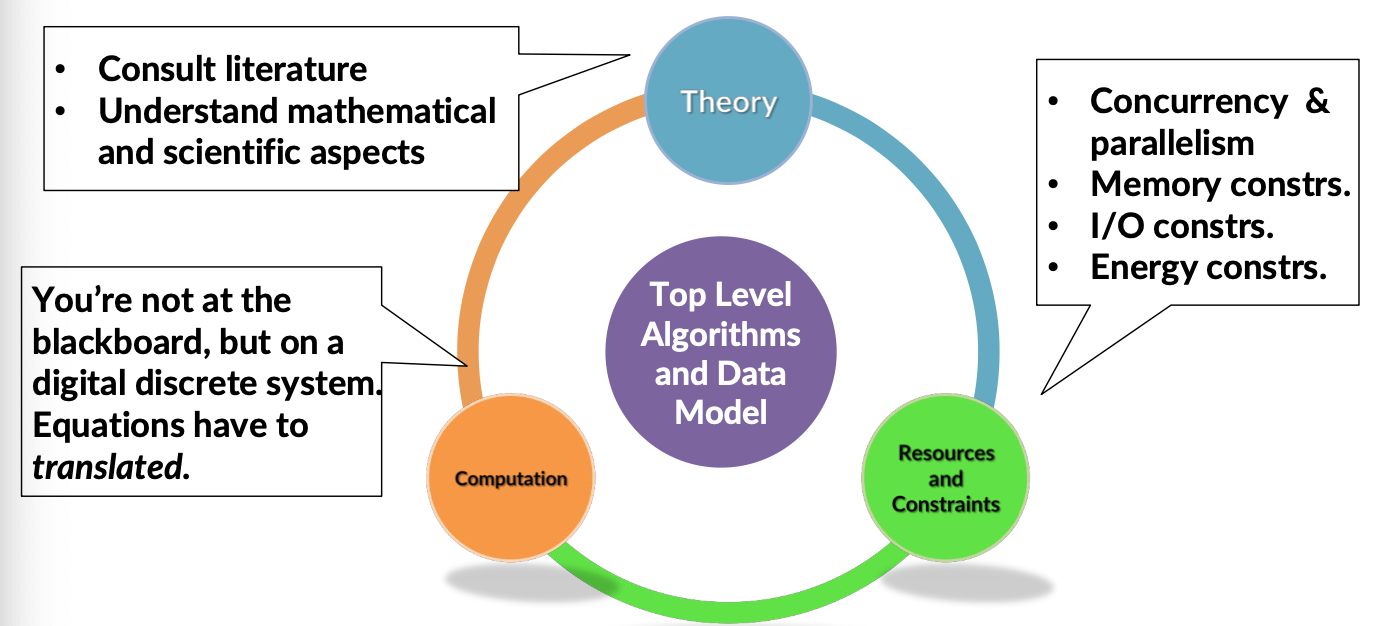
\includegraphics[width=0.7\textwidth]{assets/opt1.png}
    \caption{Optimization}
\end{figure}

\begin{itemize}
    \item \textbf{Testing} is part of the design, and it is a key step in the optimization process.
    \item \textbf{Validation} ensures that the code does what it was meant to do, and ensures the results are correct 
\end{itemize}

\newpage
\subsubsection*{First things first}
\textbf{1.} The first goal is to have a program that delivers the \textbf{correct answers} and behaves correctly under all conditions.\\
The code must be as much clear, clean, concise, and documented as possible.

\textbf{2.} The first step towards optimization is to adopt the \textbf{best-suited algorithms} and data structures. What "best-suited" means must be related to the constraints framing your activity (time-to-solution, energy-to-solution, memory, ...).

\textbf{3.} The second step is that the \textbf{source code be optimizable by the compiler}.\\
Then, you must have a firm understanding of the compiler's capabilities and limitations, as well as those of your target architecture.\\
Understand the best trade-off between portability and "performance" (accounting for the human effort into the latter).

\textbf{4.} The third step is to get a \textbf{data-driven, task-based workflow}, which possibly, almost certainly, will be parallel in either distributed- or shared-memory paradigms, or both.

\textbf{5.} Profile the code under different conditions (workload/problem size, parallelism, platforms, ...) and \textbf{spot bottlenecks and inefficiencies}.

\textbf{6.} Apply optimization techniques by modifying hot-spots in your code to \textbf{remove optimization blockers} and/or to better expose intrinsic instruction/data parallelisms.

\textbf{7.} \texttt{IF (needed) GOTO point 1.}

\vspace{1cm}
That is not a simple and linear process. Optimizing a code may require several trial-and-error steps, and modern architectures evolve so fast that modeling a code’s performance accurately can be challenging. Even promising techniques may sometimes fail.

\begin{observationblock}[Compiler job]
    Recalling the job of the compiler:
    \begin{itemize}
        \item \textbf{Syntax analysis} (parsing)
        \item \textbf{Semantic analysis} (type checking)
        \item \textbf{Intermediate code generation}
        \item \textbf{Optimization}
        \item \textbf{Code generation}
    \end{itemize}
    The compiler is a tool that can help you in the optimization process.
    
    It is also able to perform \textbf{sophisticated analysis} of the source code so that to produce a target code (usually assembly) which is highly optimized for a given target architecture.
\end{observationblock}

To optimize your code through the compiler, use \texttt{-O3} flag, where the number indicates the level of optimization.\\
\texttt{-O3} is the highest level of optimization, and it is the most aggressive one.\\
It is not granted, though, that the highest level of optimization is the best one for your code.\\
For instance, sometimes expensive optimization may generate more code that on some architecture (e.g. with smaller caches) run slower, and using \texttt{-Os} may be better.

Obviously, the compiler knows the architecture it is compiling on, but it will generate a \textbf{portable} code, i.e. a code that can run on any cpu belonging to that class of architecture. 
Using appropriate switch (in gcc \texttt{-march=native -mtune=native}), the compiler will generate code that is optimized for the specific architecture it is running on.


\textbf{Profile-guided optimization} is a technique that uses the information gathered by the compiler when the code is run to optimize the code. Compilers are able to instrument the code so to generate run-time information to be used in a subsequent compilation. 

Knowing the typical execution patterns enables the compiler to perform more focused optimizations, especially if several branches are present.
\begin{codeblock}[language=bash]
gcc -O3 -fprofile-generate -o myprog myprog.c
./myprog
gcc -O3 -fprofile-use -o myprog myprog.c
\end{codeblock}

\begin{observationblock}[Optimization blockers]
    \textbf{Optimization blockers} are those parts of the code that prevent the compiler from applying optimizations.\\
    They can be:
    \begin{itemize}
        \item \textbf{Aliasing}: when two pointers point to the same memory location
        \item \textbf{Loop-carried dependencies}: when a loop iteration depends on the result of the previous one
        \item \textbf{Function calls}: when the compiler cannot inline the function
        \item \textbf{Memory access patterns}: when the memory access pattern is not predictable
    \end{itemize}
\end{observationblock}

\subsubsection*{Memory Aliasing}

Memory Aliasing necessitates some attention.

We said that it refers to the situation where two pointers point to the same memory location.\\
This is a problem because the compiler cannot assume that the memory location is not modified by the other pointer, and it must reload the value from memory each time it is accessed.
Help your C compiler in doing the best effort, either writing a clean code or using restrict or using \texttt{-fstrict-aliasing -Wstrict-aliasing} options.

\begin{exampleblock}[Memory aliasing]
    \begin{codeblock}[language=C++]
        void my_fun(double *a, double *b, int n) {
            for (int i = 0; i < n; i++) {
                a[i] = b[i] + 1.0;
            }
        }

        // can be optimized to
        void my_fun(double *restrict a, double *restrict b, int n) {
            for (int i = 0; i < n; i++) {
                a[i] = b[i] + 1.0;
            }
        }
    \end{codeblock}
    Now you are telling the compiler that the memory regions
    referenced by a and b will never overlap.
    So, it will feel confident in optimizing the memory accesses as
    much as it can (basically avoiding to re-read locations).
\end{exampleblock}



\newpage
\subsection{Modern Architectures}

This section presents the fundamental traits of the \textbf{single-core} modern architectures.

\begin{figure}[H]
    \centering
    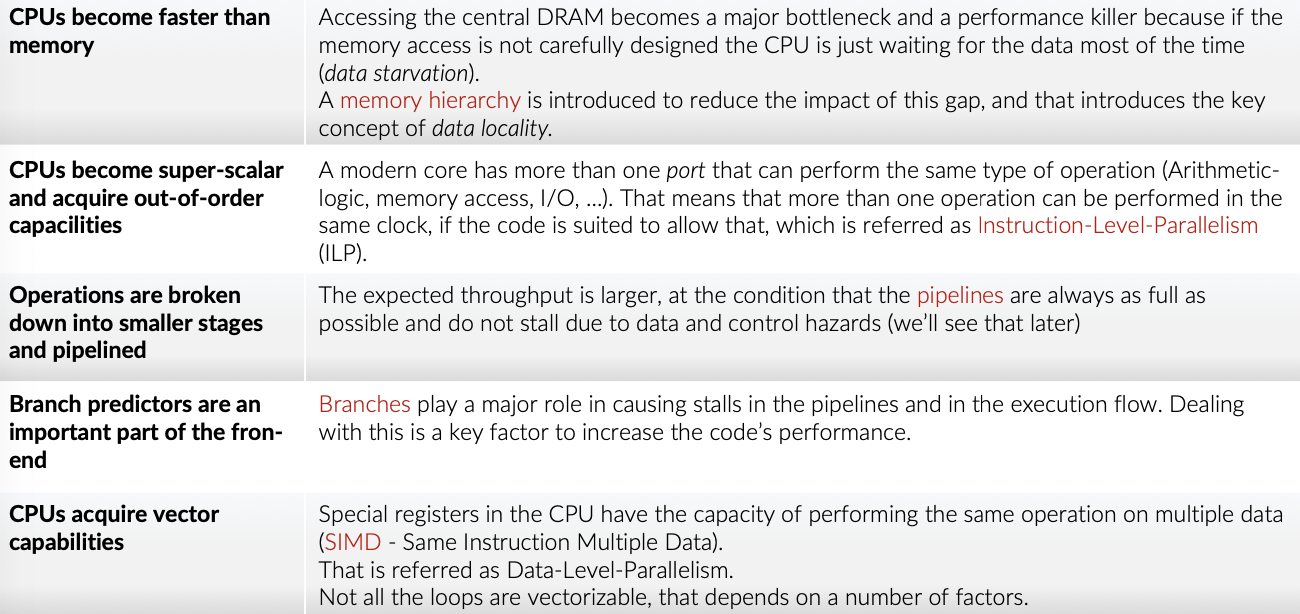
\includegraphics[width=0.9\textwidth]{assets/opt2.png}
    \caption{At a glance}
\end{figure}

In the \textbf{Von Neumann} architecture there is only 1 processing unit, 1 instruction is executed at a time and the memory is "flat".  It was much simpler than today's architectures, but it is still the basis of modern computers.

\begin{figure}[H]
    \centering
    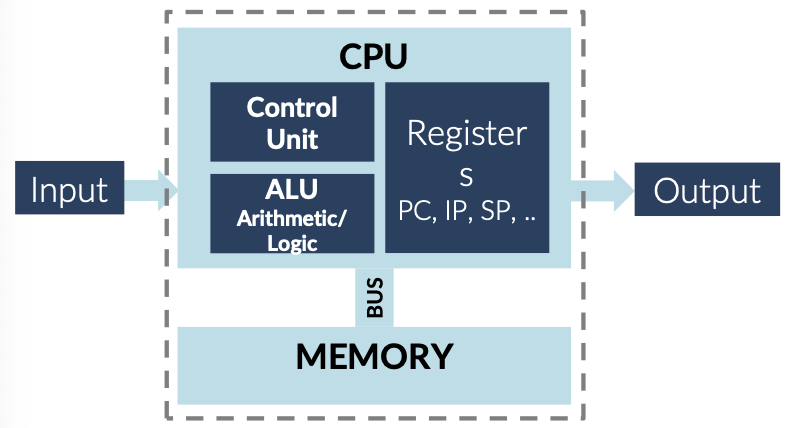
\includegraphics[width=0.6\textwidth]{assets/opt3.png}
    \caption{Von Neumann architecture}
\end{figure}
        
Today, instead:
\begin{itemize}
    \item there are many processing UniTs
    \item many instructions can be executed at a time 
    \item many data can be processed at a time 
    \item "instructions" are internally broken down into many simpler operations that are pipelined 
    \item memory is strongly not "flat", there is a strong memory hierarchy, access memory can have very differnt costs depending on the location and accessing RAM is way more costly than performing operations on internal registers.
\end{itemize}

We have seen that the power required per transistor is 
\[
    C \times V^2 \times f   
\]

Roughly the capacitance and the voltage of transistor shrinks with the feature size, whereas the scaling is much more complicated for the wires. Overall, a typical CPU got from ~2W power to ~100W which is at the limit of the air cooling capacity. 

To cope with the power wall one can:
\begin{itemize}
    \item Turn off inactive circuits 
    \item Downscale Voltage and Frequency for both cores and DRAM 
    \item Thermal Power Design, or design for typical case 
    \item Overclocking for a short period of time and possibly for just a fraction of the chip
\end{itemize}

\vspace{0.5cm}
\textbf{CPU became faster than memory in the early 90s}.

The CPU may spend more time waiting for data coming from RAM than executing operations. That is part of the so called "memory wall". The solution is to use a memory hierarchy, where the data is stored in different levels of memory, each one with different access times and sizes.
Furthermore, to be faster it ought to be extremelty closer. The new memory that will be called \textbf{cache}, will be much smaller than the RAM.

The cache itself has a hierarchy:
\begin{itemize}
    \item L1 cache: very small, very fast, very close to the core
    \item L2 cache: bigger, slower, still close to the core
    \item L3 cache: bigger, slower, shared among cores
\end{itemize}

\begin{figure}[H]
    \centering
    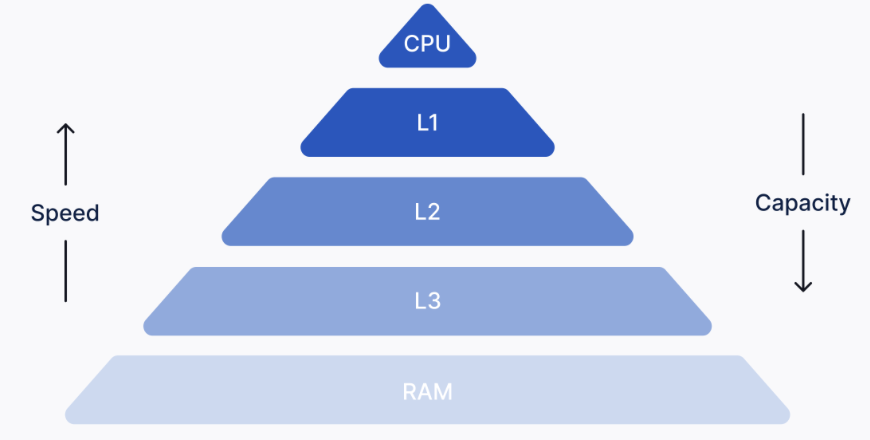
\includegraphics[width=0.6\textwidth]{assets/opt4.png}
    \caption{Memory hierarchy}
\end{figure}

\begin{definitionblock}[Principle of Locality]
    Data are defined "local" when they reside in a small portion of the address space that is accessed in some short period of time.

    There are two types of locality:
    \begin{itemize}
        \item \textbf{Temporal locality}: if an item is referenced, it will tend to be referenced again soon.
        \item \textbf{Spatial locality}: if an item is referenced, items whose addresses are close by will tend to be referenced soon.
    \end{itemize}
\end{definitionblock}





\newpage
\section{Cache Hierarchy}

The RAM contains ~$10^9$ bytes, while L1 contains ~$10^4$ bytes (32KB for data and 32KB for instructions). So, how do we map the RAM into a given level of cache, for instance L1, in an effective way?

\begin{itemize}
    \item Where to map an address?
    \item What if the location in L1 is already occupied?
\end{itemize}

Let's say that both the RAM and the cache are subdivided in blocks of equal size (64B): you do not load just a byte in your cache, but an entire block (called \textit{line})
\begin{figure}[H]
    \centering
    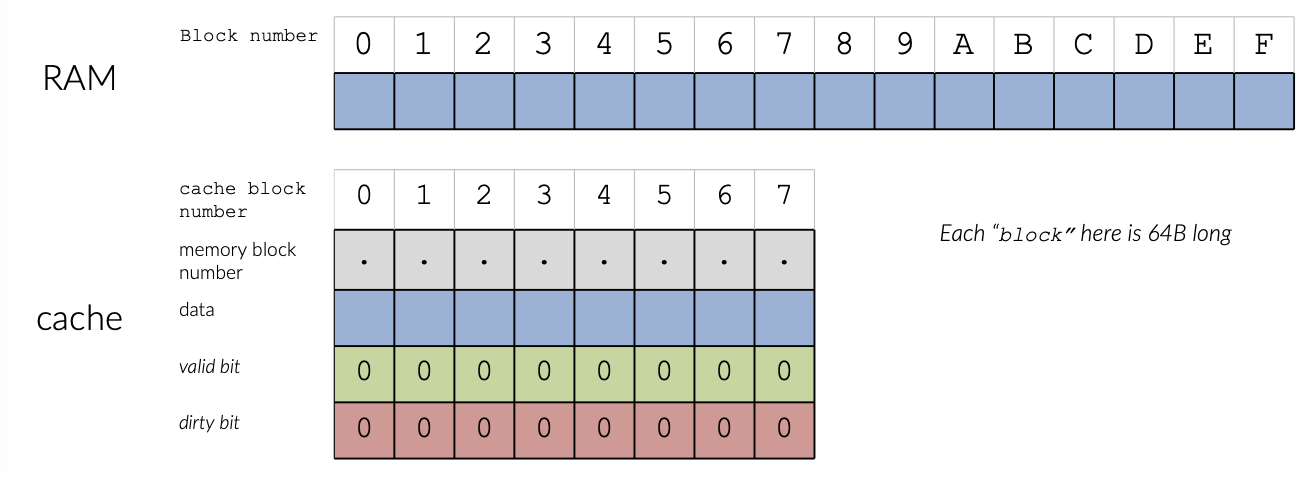
\includegraphics[width=0.6\textwidth]{assets/opt5.png}
    \caption{Cache hierarchy}
\end{figure}

There exist three main strategies to map the RAM into the cache:
\begin{itemize}
    \item \textbf{Full mapping}: Data can be placed in any free cache block. This is the simplest strategy, but it is not efficient.
    \begin{figure}[H]
        \centering
        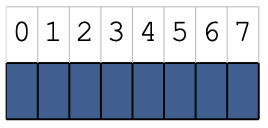
\includegraphics[width=0.3\textwidth]{assets/opt6.png}
        \caption{Full mapping}
    \end{figure}
    \item \textbf{Direct mapping}: Each block of RAM can be placed in only one block of the cache. This is a simple strategy, but it is not efficient.
    \begin{figure}[H]
        \centering
        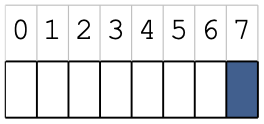
\includegraphics[width=0.3\textwidth]{assets/opt7.png}
        \caption{Direct mapping}
    \end{figure}
    \item \textbf{n-way associative}: Each block of RAM can be placed in a set of n blocks of the cache. This is a more complex strategy, but it is more efficient.
    \begin{figure}[H]
        \centering
        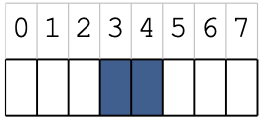
\includegraphics[width=0.3\textwidth]{assets/opt8.png}
        \caption{n-way associative}
    \end{figure}
\end{itemize}

\begin{table}[H]
\centering
\caption{Cache Mapping Strategies}
\begin{tabular}{l p{3.5cm} p{2.8cm} p{2.8cm}}
\toprule
\textbf{Strategy} & \textbf{Description} & \textbf{Pros} & \textbf{Cons} \\
\midrule
Full mapping 
& Any block can store any address 
& Very flexible, good space use
& More complex to search, higher hardware cost \\
\addlinespace
Direct mapping 
& Each address maps to exactly one cache block 
& Simple design, fast lookups
& Higher chances of conflicts, limited flexibility \\
\addlinespace
n-way associative 
& Cache is divided into sets of n blocks 
& Balances speed and flexibility 
& More complex than direct mapping \\
\bottomrule
\end{tabular}
\end{table}

\begin{figure}[H]
    \centering
    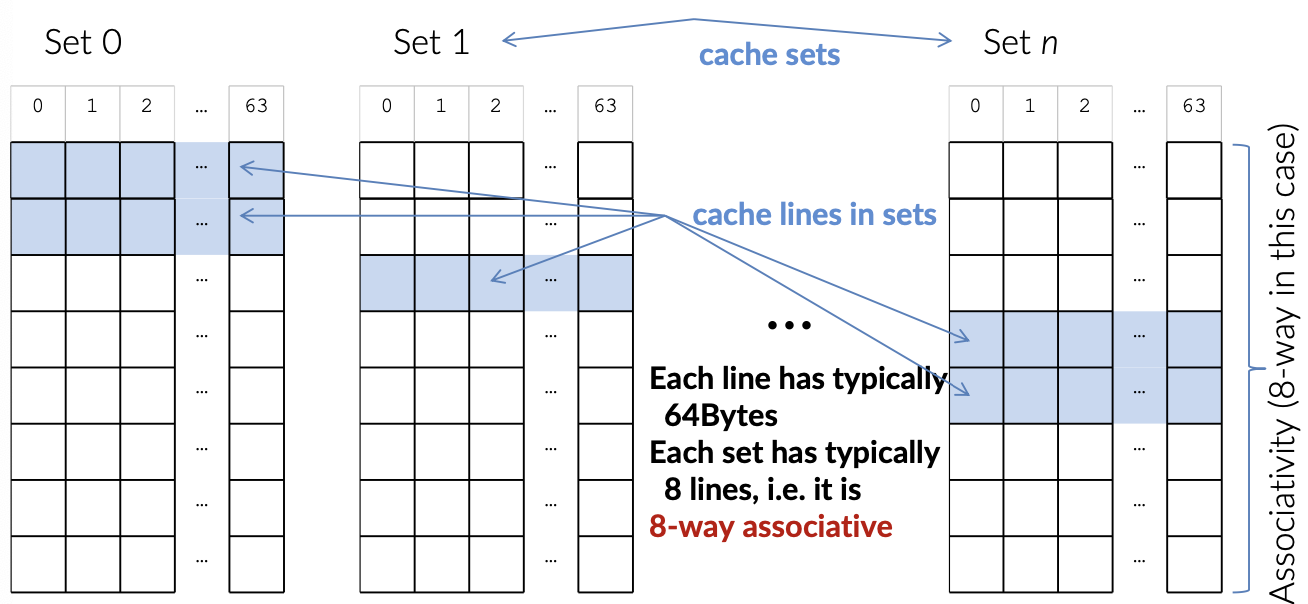
\includegraphics[width=0.9\textwidth]{assets/opt9.png}
    \caption{A typical today cache}
\end{figure}

\begin{advancedblock}[Cache mapping]
    \textbf{How a byte is actually mapped into a cache location?}


\end{advancedblock}

\subsection*{The memory access pattern}

Consider a simple direct mapped \textbf{16 byte data cache} with \textbf{two cache lines}, each of size 8B. 

Consider the following code sequence, in which the array \texttt{X} is cache-aligned (i.e., \texttt{x[0]} is always loaded into the beginning of the first cache line) and accessed twice in consecutive order:

\begin{figure}[H]
    \centering
    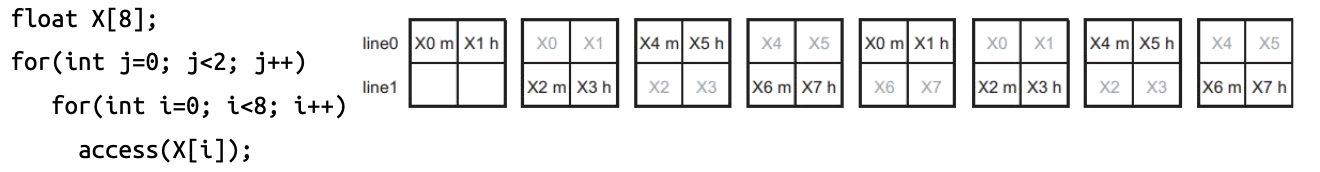
\includegraphics[width=0.9\textwidth]{assets/opt10.png}
    \caption{The hit-miss pattern is: MH MH MH MH MH MH MH MH, the miss-rate is 50\% (the first miss is compulsory miss)}
\end{figure}

Let's consider another code sequence that access the array twice as before, but with a strided access.

\begin{figure}[H]
    \centering
    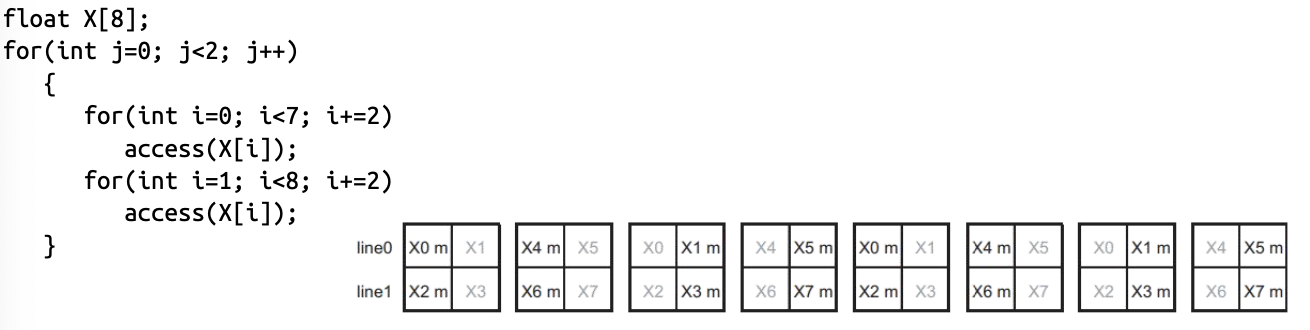
\includegraphics[width=0.9\textwidth]{assets/opt11.png}
    \caption{The hit-miss pattern now is: MM MM MM MM MM MM MM MM, the miss-rate is 100\%}
\end{figure}

Finally, consider a third code sequence that again access the array twice:
\begin{figure}[H]
    \centering
    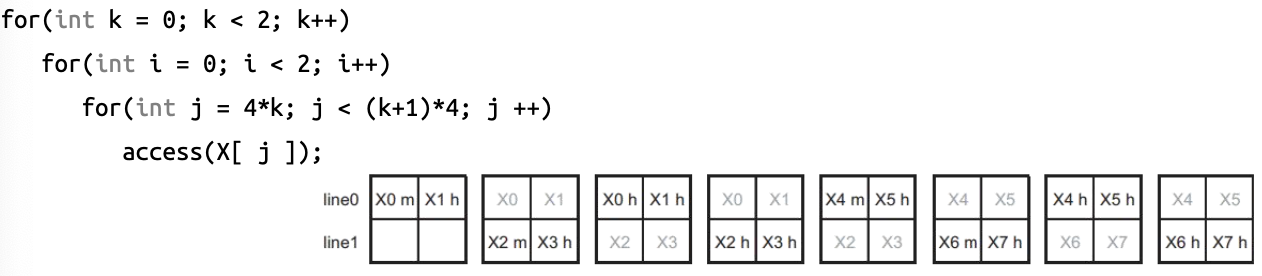
\includegraphics[width=0.9\textwidth]{assets/opt12.png}
    \caption{The hit-miss pattern now is: MH MH HH HH MH MH HH HH, the miss-rate is 25\%}
\end{figure}

